%%%%%%%%%%%%%%%%%%%%%%%%%%%%%%%%%%%%%%%%%%%%%%%%%%%%%%%%%%%%%%%
% Welcome to the MAT320 Homework template on Overleaf -- just edit your
% LaTeX on the left, and we'll compile it for you on the right.
%%%%%%%%%%%%%%%%%%%%%%%%%%%%%%%%%%%%%%%%%%%%%%%%%%%%%%%%%%%%%%%
% --------------------------------------------------------------
% Based on a homework template by Dana Ernst.
% --------------------------------------------------------------
% This is all preamble stuff that you don't have to worry about.
% Head down to where it says "Start here"
% --------------------------------------------------------------

\documentclass[12pt]{article}

\usepackage{graphicx}
\graphicspath{{./images/}}
\usepackage{textcomp} % cent symbol, such as \textcent
\usepackage[margin=1in]{geometry} 
\usepackage{amsmath,amsthm,amssymb}
\usepackage{mathtools} % ceiling function
\DeclarePairedDelimiter{\ceil}{\lceil}{\rceil}
% https://tex.stackexchange.com/questions/146306/how-to-make-horizontal-lists
\usepackage[inline]{enumitem} % allows using letters in enumerate list environment

% source: https://stackoverflow.com/questions/3175105/inserting-code-in-this-latex-document-with-indentation

\usepackage{listings}
\usepackage{color}

\definecolor{dkgreen}{rgb}{0,0.6,0}
\definecolor{gray}{rgb}{0.5,0.5,0.5}
\definecolor{mauve}{rgb}{0.58,0,0.82}

\lstset{frame=tb,
	language=VHDL, % language for code listing
	aboveskip=3mm,
	belowskip=3mm,
	showstringspaces=false,
	columns=flexible,
	basicstyle={\small\ttfamily},
	numbers=none,
	numberstyle=\tiny\color{gray},
	keywordstyle=\color{blue},
	commentstyle=\color{dkgreen},
	stringstyle=\color{mauve},
	breaklines=true,
	breakatwhitespace=true,
	tabsize=4
}

\newcommand{\N}{\mathbb{N}}
\newcommand{\Z}{\mathbb{Z}}

\newenvironment{ex}[2][Exercise]{\begin{trivlist}
		\item[\hskip \labelsep {\bfseries #1}\hskip \labelsep {\bfseries #2.}]}{\end{trivlist}}

\newenvironment{sol}[1][Solution]{\begin{trivlist}
		\item[\hskip \labelsep {\bfseries #1:}]}{\end{trivlist}}


\begin{document}

% --------------------------------------------------------------
%                         Start here
% --------------------------------------------------------------

\noindent Sergio Garcia Tapia \hfill

\noindent{\small Digital Design and Computer Architecture: RISC-V, by
Sarah and David Harris} \hfill

\noindent{\small Chapter 5: Digital Building Blocks} \hfill 

\noindent\today

\begin{ex}{5.1}
	What is the delay for the following types of $64$-bit adders? Assume
	that each two-input gate delay is $150$ ps and that a full adder delay
	is $450$ ps.
	\begin{enumerate}[label=(\alph*)]
		\item a ripple-carry adder
		\item a carry-lookahead adder with 4-bit blocks
		\item a prefix adder
	\end{enumerate}
\end{ex}

\begin{sol}
	\
	\begin{enumerate}[label=(\alph*)]
		\item The delay of a ripple-carry adder is governed by
		the equation
		\begin{align*}
			t_{\text{ripple}}=Nt_{FA}
		\end{align*}
		where $N$ is the number of full adders chained together, and $t_{FA}$ is the delay
		of a full adder. Since a full adder is a two-input gate, the assumption is that
		$t_{FA}=150$ ps. Moreover, since the adder deals with $64$-bit, we have $N=64$.
		Therefore the delay is:
		\begin{align*}
			t_{\text{ripple}}=64\cdot 450 \text{ ps } =  28800 \text{ ps } = 288 \text{ ns}.
		\end{align*}
		\item The delay of a carry-lookahead adder with $k$-bit blocks is governed by
		the equation
		\begin{align*}
			t_{CLA}=t_{pg}+t_{pg\_\text{block}}+\left(\frac{N}{k}-1\right)t_{\text{AND\_OR}}+kt_{FA},
		\end{align*}
		where $t_{pg}$ is the delay of the column propagate and generates (which is a single
		AND or OR gate) to generate $P_i$ and $G_i$, $t_{pg\_\text{block}}$ is the delay to find
		the block propagate and generate signals $P_{i:j}$ and $G_{i:j}$ for a $k$-bit block,
		and $t_{\text{AND\_OR}}$ is the delay from $C_{\text{in}}$ to $C_{\text{out}}$ through
		the final AND/OR logic of the $k$-bit CLA block. Hence, the critical path is as follows
		\begin{enumerate}[label=(\roman*)]
			\item Compute all column generate and propagate signals $P_i$ and $G_i$
			in parallel for all blocks; since they all go through AND or OR, this
			costs $t_{pg}=150$ ps delay.
			\item Compute all block generate and propagate signals, $P_{i:j}$ and
			$G_{i:j}$, where the critical path goes into computing $G_{i:j}$. For
			4-bit blocks, this consists of 6 AND/OR gates, so
			$t_{pg\_\text{block}}=6\cdot 150\text { ps }=900\text{ ps}$.
			\item Compute $C_{out}$ using $G_{i:j}$ and the already-computed result
			of $C_{in}P_{i:j}$. This computes $C_{out}$, which is $C_3$, and then
			it goes through the rest of the blocks until it reaches the last one.
			The total cost is thus $\left(\frac{64}{4}-1\right)t_{\text{AND\_OR}}=15\cdot 150 \text{ ps }=
			2250\text{ ps }$.
			\item The last on the critical path is the cost of the ripple-carry adder
			that consists of four full adders, each of which has three 2-input gates in its
			critical path. Therefore, $kt_{FA}=4\cdot (3\cdot 150 \text{ ps })=1800\text{ ps}$.
			We finally have
			\begin{align*}
				t_{CLA}&=150\text{ ps} + 900\text{ ps} + 2250\text{ ps } + 1800\text{ ps}=5100\text{ ps}=
				5.1\text{ ns}.
			\end{align*}
		\end{enumerate}
		\item The equation governing the delay of a prefix adder is
		\begin{align*}
			t_{PA}=t_{pg}+\log_2N(t_{pg\_\text{prefix}})+t_{\text{XOR}}
		\end{align*}
		where $t_{pg}$ is the precomputation delay of all $P_i$ and $G_i$ (which happens in parallel and
		costs a single 2-input gate), $t_{pg\_\text{prefix}}$ is the delay of a prefix cell,
		and $t_{\text{XOR}}$ is the delay due to the final XOR gate to compute $S_i$.
		Note that the critical path delay for a single prefix block is two 2-input gates
		to compute $G_{i:j}$. Hence, the total delay is
		\begin{align*}
			t_{PA}&=150\text{ ps} + \log_2 64\cdot (300\text{ ps})+150\text{ ps}=2100\text{ ps}=2.1\text{ ns}.
		\end{align*}
	\end{enumerate}
\end{sol}
                                               
\begin{ex}{5.3}
	Explain why a designer might choose to use a ripple-carry adder instead
	of a carry look-ahead adder.
\end{ex}

\begin{sol}
	A designer may want a less complex circuit, which they can get by using a ripple-carry
	adder. Related, they may also be looking to use less hardware and/or power. Their
	specifications may not require the speed improvements that they would get by
	using a carry-lookahead adder.
\end{sol}

\begin{sol}
\end{sol}

\begin{ex}{5.5}
	The prefix network shown in Figure ~\ref{16-bit-prefix-adder-schematic} uses black cells to compute all of the
	prefixes.
	\begin{figure}
		\centering
		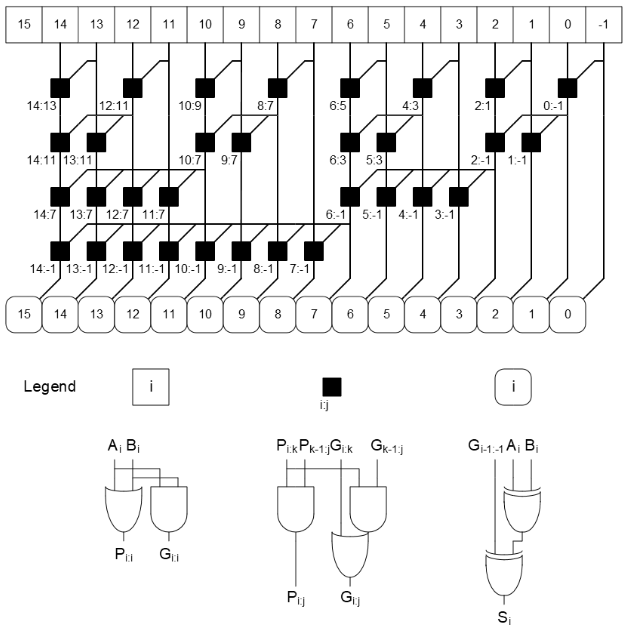
\includegraphics[width=0.8\textwidth]{16-bit-prefix-adder-schematic}
		\caption{16-bit prefix adder}
		\label{16-bit-prefix-adder-schematic}
	\end{figure}
	
	Some of the block propagate signals are not actually necessary. Design a
	``gray cell" that receives $G$ and $P$ signals for bits $i$:$k$ and $k-$1:$j$ but
	produces only $G_{i:j}$, not $P_{i:j}$. Redraw the prefix network, replacing black
	cells with gray cells wherever possible.
\end{ex}

\begin{sol}
	See Figure~\ref{16-bit-prefix-adder-grey-cells}. To understand it, note that
	in the second level, all cells depend on cells from on a $P_{i:j}$ value
	from the first level, so all blocks must be black.
	In the third level, $G_{5:-1}$ and $G_{6:-1}$ both depend on $P_{2:-1}$, so
	that corresponding cell must be black. On the other hand, none of the cells
	in the third level depend on $P_{1:-1}$. In the fourth level,
	all cells, which comptue $G_{7:-1},\ldots, G_{14:-1}$, depend on $P_{6:-1}$,
	so the corresponding block must be black.
	\begin{figure}
		\centering
		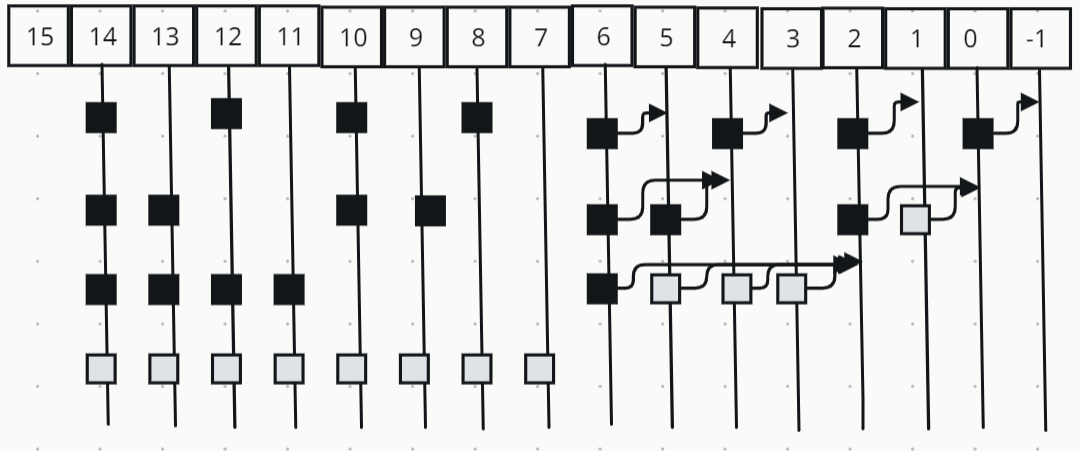
\includegraphics[width=0.7\textwidth]{16-bit-prefix-adder-grey-cells}
		\caption{Exercise 5.8: 16-bit prefix adder with ``grey cells".}
		\label{16-bit-prefix-adder-grey-cells}
	\end{figure}
\end{sol}

\begin{ex}{5.8}
	Design the following comparators for $32$-bit unsigned numbers. Sketch the schematics.
	\begin{enumerate}[label=(\alph*)]
		\item not equal
		\item greater than or equal to
		\item less than
	\end{enumerate}
\end{ex}

\begin{sol}
	\
	\begin{enumerate}[label=(\alph*)]
		\item See Figure~\ref{unequal-32-bit-unsigned-comparator}. We take the
		XOR of $A_iB_i$, and then OR all results.
		\begin{figure}
			\centering
			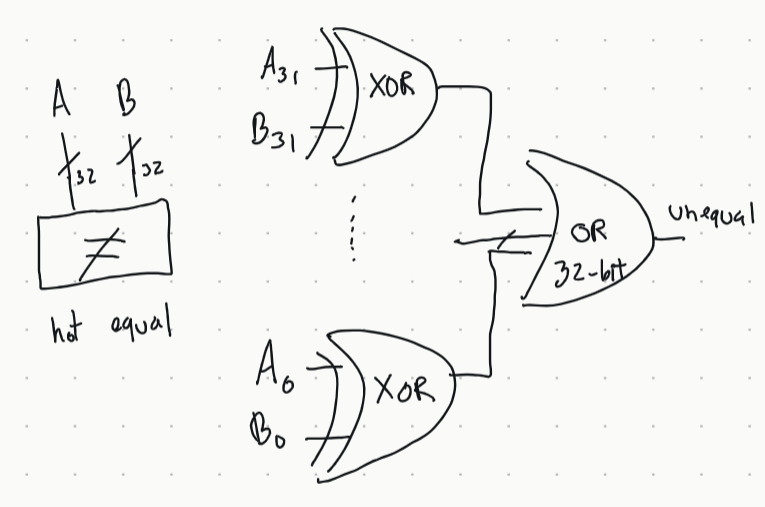
\includegraphics[width=0.6\textwidth]{unequal-32-bit-unsigned-comparator}
			\caption{Exercise 5.8: 32-bit unequal unsigned comparator}
			\label{unequal-32-bit-unsigned-comparator}
		\end{figure}
		\item See Figure~\ref{greater-than-or-equal-to-32-bit-unsigned-comparator}.
		We subtract, and if the most significant bit is 0, then $A\geq B$.
		\begin{figure}
			\centering
			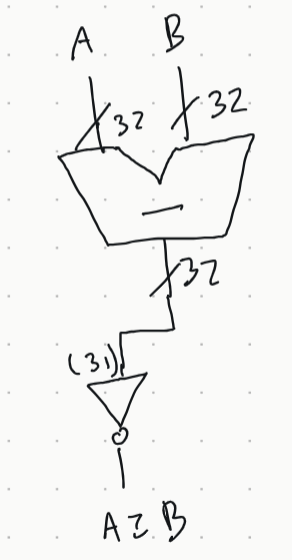
\includegraphics[width=0.2\textwidth]{greater-than-or-equal-to-32-bit-unsigned-comparator}
			\caption{Exercise 5.8: 32-bit greater than or equal to unsigned comparator}
			\label{greater-than-or-equal-to-32-bit-unsigned-comparator}
		\end{figure}
		\item See Figure~\ref{less-than-32-bit-unsigned-comparator}. We subtract,
		and if the most significant bit is $1$, then $A<B$.
		\begin{figure}
			\centering
			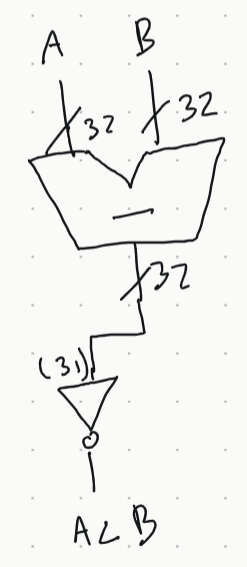
\includegraphics[width=0.2\textwidth]{less-than-32-bit-unsigned-comparator}
			\caption{Exercise 5.8: 32-bit less than unsigned comparator}
			\label{less-than-32-bit-unsigned-comparator}
		\end{figure}
	\end{enumerate}
\end{sol}

\begin{ex}{5.9}
	Consider the signed comparator of Figure~\ref{signed-comparator}.
	\begin{figure}
		\centering
		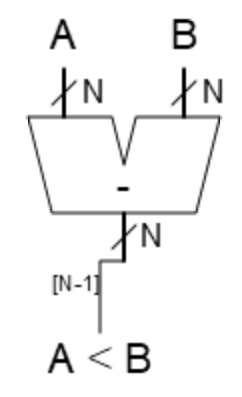
\includegraphics[width=0.2\textwidth]{signed-comparator}
		\caption{$N$-bit signed comparator}
		\label{signed-comparator}
	\end{figure}
	\begin{enumerate}[label=(\alph*)]
		\item Give an example of two 4-bit signed numbers $A$ and $B$ for which a 4-bit
		signed comparator correctly computes $A<B$.
		\item Give an example of two 4-bit signed numbers $A$ and $B$ for which a 4-bit
		signed comparator incorrectly computes $A<B$.
		\item In general, when does the $N$-bit signed comparator operator incorrectly?
	\end{enumerate}
\end{ex}

\begin{sol}
	\begin{enumerate}[label=(\alph*)]
		\item It operates correctly on $A=0_2=0=0000$ and $B=1_2=0001$.
		\item It operates incorrectly on $A=7_2=0111$ and $B=(-1)_2=1111$.
		\item As mentioned in the text, it operates incorrectly when there
		is overflow. Specifically, if $A$ and $B$ have opposite signs and
		the sign of the output $S$ is not the same sign as $A$.
	\end{enumerate}
\end{sol}

\begin{ex}{5.10}
	Modify the $N$-bit signed comparator of Figure~\ref{signed-comparator} to operate
	correctly when $A<B$ for all $N$-bit signed inputs $A$ and $B$.
\end{ex}

\begin{sol}
	As discussed in Exercise 5.9, the ``less than" signed comparator computes $A<B$ incorrectly
	when $A$ and $B$ have opposite signs and the sign of the output $S$ is not the same as the
	sign of $A$; this indicates overflow has occurred. Letting $V$ be the overflow
	signal and $Y$ be the less-than signal, their equations are
	\begin{align*}
		V&=A_{31}\bar{B}_{31}\bar{S}_{31}+\bar{A}_{31}B_{31}S_{31};\\
		Y&=V\oplus S.
	\end{align*}
	See Figure~\ref{unsigned-comparator-overflow-accounted}.
	\begin{figure}
		\centering
		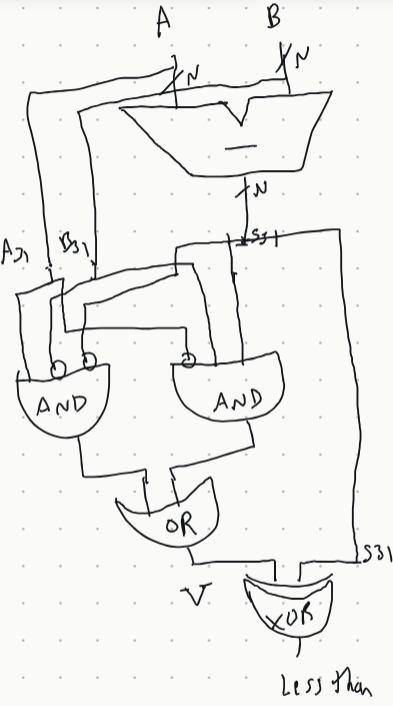
\includegraphics[width=0.4\textwidth]{unsigned-comparator-overflow-accounted}
		\caption{Unsigned $N$-bit comparator that accounts for overflow}
		\label{unsigned-comparator-overflow-accounted}
	\end{figure}
\end{sol}

\begin{ex}{5.11}
	Design the 32-bit ALU shown in Figure~\ref{n-bit-ALU} using your favorite HDL.
	You can make the to-level module either behavior or structural.
	\begin{figure}
		\centering
		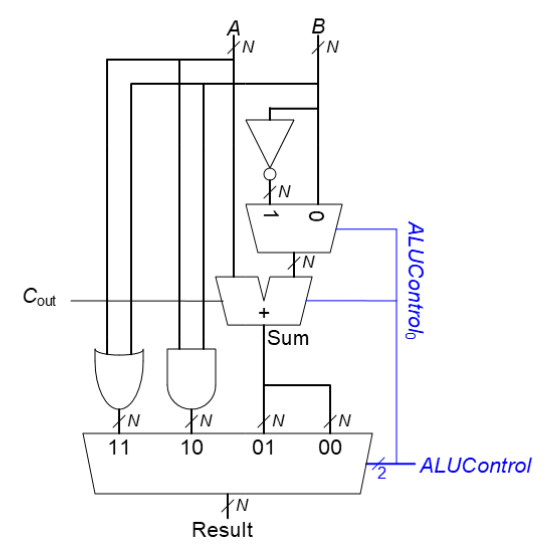
\includegraphics[width=0.5\textwidth]{n-bit-ALU}
		\caption{$N$-bit ALU}
		\label{n-bit-ALU}
	\end{figure}
\end{ex}

\begin{sol}
	See code listing for \texttt{./hdl/11-alu-32/alu\_32.vhd}:
	\lstinputlisting{./hdl/11-alu-32/alu_32.vhd}
\end{sol}

\begin{ex}{5.12}
	Design the 32-bit ALU shown in Figure~\ref{n-bit-ALU-flags} using your favorite HDL.
	You can make the to-level module either behavior or structural.
	\begin{figure}
		\centering
		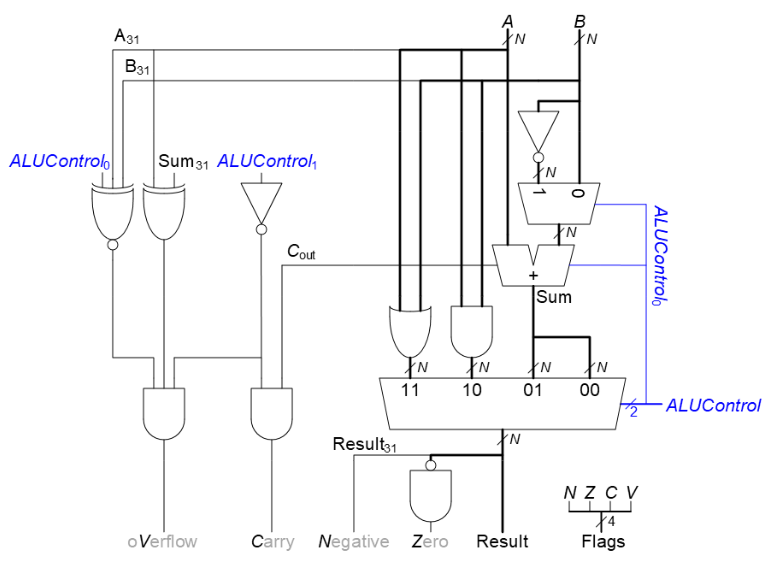
\includegraphics[width=0.7\textwidth]{n-bit-ALU-flags}
		\caption{$N$-bit ALU with flags}
		\label{n-bit-ALU-flags}
	\end{figure}
\end{ex}

\begin{sol}
	See code listing for \texttt{./hdl/12-alu-32-flags/alu\_32\_flags.vhd}:
	\lstinputlisting{./hdl/12-alu-32-flags/alu_32_flags.vhd}
\end{sol}

\begin{ex}{5.13}
	Design the 32-bit ALU shown in Figure~\ref{n-bit-ALU-set-if-less-than}~(a) 
	using your favorite HDL. You can make the to-level module either behavior or structural.
	\begin{figure}
		\centering
		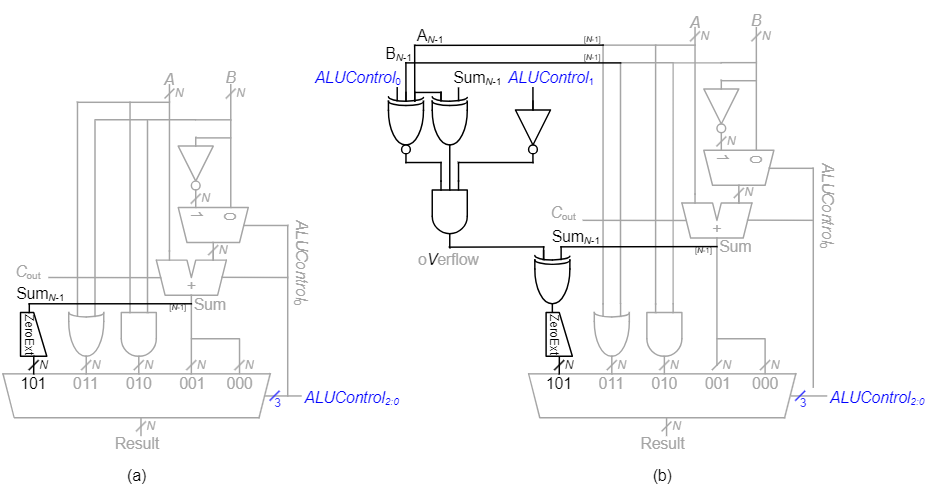
\includegraphics[width=0.9\textwidth]{n-bit-ALU-set-if-less-than}
		\caption{$N$-bit ALU with flags}
		\label{n-bit-ALU-set-if-less-than}
	\end{figure}
\end{ex}

\begin{sol}
	See code listing for \texttt{./hdl/13-alu-32-slt/alu\_32\_slt.vhd}:
	\lstinputlisting{./hdl/13-alu-32-slt/alu_32_slt.vhd}
\end{sol}

\begin{ex}{5.14}
	Design the 32-bit ALU shown in Figure~\ref{n-bit-ALU-set-if-less-than}~(b)  using your favorite HDL.
	You can make the to-level module either behavior or structural.
\end{ex}

\begin{sol}
	See code listing for
	\texttt{./hdl/14-alu-32-slt-overflow/alu\_32\_slt\_overflow.vhd}:
	\lstinputlisting{./hdl/14-alu-32-slt-overflow/alu_32_slt_overflow.vhd}
\end{sol}

\begin{ex}{5.19}
	Build an \emph{unsigned comparison unit} that compares two unsigned numbers $A$ and $B$.
	The unit's input is the \emph{Flags} signal ($N, Z, C, V$) from the ALU of
	Figure~\ref{5.16}, with the ALU performing subtraction: $A-B$. The unit's outputs
	are $HS, LS, HI$, and $LO$, which indicate that $A$ is higher than or the same as
	($HS$), lower than or the same as ($LS$), high ($HI$), or lower ($LO$) than $B$.
	\begin{enumerate}[label=(\alph*)]
		\item Write minimal equations for $HS, LS, HI$ and $LO$ in terms of $N, Z, C$,
		and $V$.
		\item Sketch circuits for $HS,LS,HI$, and $LO$.
	\end{enumerate}
\end{ex}

\begin{sol}
	\begin{enumerate}[label=(\alph*)]
		\item As discussed in the text, when using the subtraction of two inputs
		$A$ and $B$ to do comparison, we know that $A<B$ if there is no carry.
		On the other hand, $A\geq B$ is there is a carry. We can then use
		the zero signal to know whether it can be less than or equal to or greater
		than. The $N$ and $V$ signals are don't-cares. The equations are below:
		\begin{align*}
			HS=C,\quad LS=Z+C,\quad HI=\bar{Z}C,\quad LO=\bar{C}
		\end{align*}
		\item See the sketch in Figure~\ref{unsigned-comparison-unit}.
		\begin{figure}
			\centering
			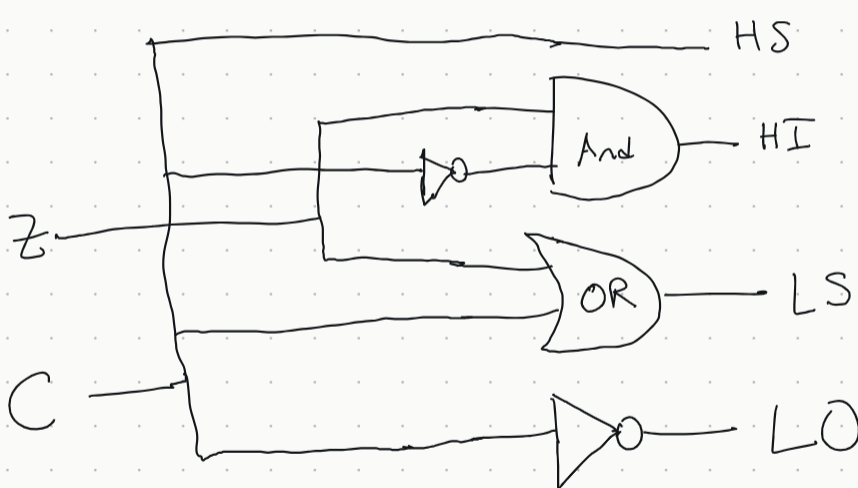
\includegraphics[width=0.5\textwidth]{exercise-05-19-unsigned-comparison-unit}
			\caption{Exercise 5-19: Unsigned Comparison Unit}
			\label{unsigned-comparison-unit}
		\end{figure}
	\end{enumerate}
\end{sol}

\begin{ex}{5.20}
	Build an \emph{signed comparison unit} that compares two unsigned numbers $A$ and $B$.
	The unit's input is the \emph{Flags} signal ($N, Z, C, V$) from the ALU of
	Figure~\ref{5.16}, with the ALU performing subtraction: $A-B$. The unit's outputs
	are $GE, LE, GT$, and $LT$, which indicate that $A$ is greater than or equal to
	($GE$), less than or equal to ($LE$), greater than ($GT$), or less than ($LT$) than $B$.
	\begin{enumerate}[label=(\alph*)]
		\item Write minimal equations for $GE, LE, GT$ and $LT$ in terms of $N, Z, C$,
		and $V$.
		\item Sketch circuits for $GE,LE,GT$, and $LT$.
	\end{enumerate}
\end{ex}

\begin{sol}
	\begin{enumerate}[label=(\alph*)]
		\item As discussed in the text, the $N$ (negative) flag communicates
		that $A-B$ is negative. But to use it for signed magnitude comparison,
		we must also use the $V$ flag to account for overflow. The equations
		are below:
		\begin{align*}
			LT=N\oplus V,\quad GE=\overline{N\oplus V},
			\quad LE=Z+N\oplus V,\quad GT=\bar{Z}\cdot \overline{N\oplus V}
		\end{align*}
		\item See the sketch in Figure~\ref{signed-comparison-unit}.
		\begin{figure}
			\centering
			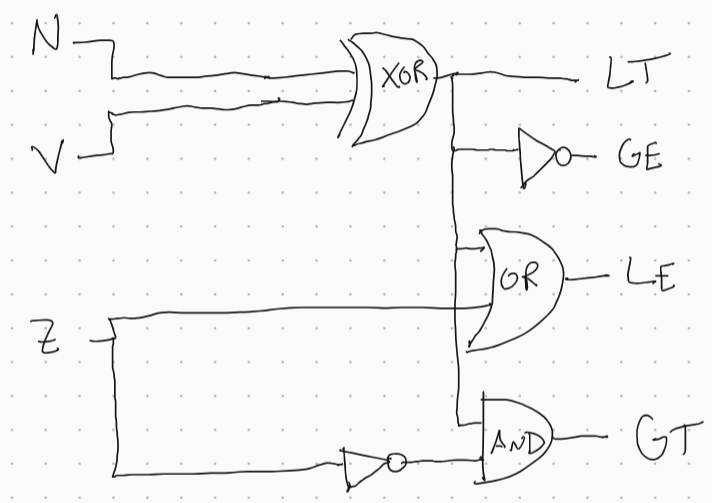
\includegraphics[width=0.5\textwidth]{exercise-05-20-signed-comparison-unit}
			\caption{Exercise 5-20: signed Comparison Unit}
			\label{signed-comparison-unit}
		\end{figure}
	\end{enumerate}
\end{sol}

\begin{ex}{5.21}
	Design a shifter that always shifts a 32-bit input left by 2 bits. The input and
	output are both 32 bits. Explain the design in words and sketch a schematic.
	Implement your design in your favorite HDL.
\end{ex}

\begin{sol}
	When the input $A$ is shifted left by 2, the output will always receive 0 in its
	two least significant fits. See the sketch in Figure~ref{exercise-21-32bit-shift-left-2}.
	\begin{figure}
		\centering
		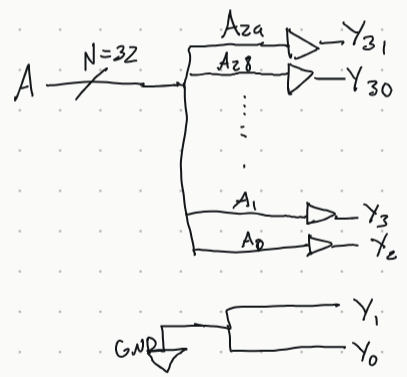
\includegraphics[width=0.4\textwidth]{exercise-21-32bit-shift-left-2}
		\caption{Exercise 21: Shifter that always shifts its 32-bit input left by
		2 bits.}
		\label{exercise-21-32bit-shift-left-2}
	\end{figure}
	See code listing for
	\texttt{./hdl/21-shifter-left-32bit-2/shifter\_left\_32bit\_2.vhd}:
	\lstinputlisting{./hdl/21-shifter-left-32bit-2/shifter_left_32bit_2.vhd}
\end{sol}

\begin{ex}{5.24}
	Explain how to build any $N$-bit shifter or rotator using only $N\log_2N$ 2:1
	multiplexers.
\end{ex}

\begin{sol}
	Given an $N$-bit input, we also accept a $\log_2 N$-bit input named $shamt$
	which indicates the amount by which to shift. If we could use $N:1$ multiplexers,
	then $N$ such multiplexers, each with the $shamt$ input as its select signal.
	To build an $N:1$ multiplexer, we need $log_2N$ $2:1$ multiplexers. Therefore,
	the $N$ multiplexers, each $N:1$, would take $N\log_2N$ $2:1$ multiplexers.
	\
	
	Consider the left shift case. Arrange the $N:1$ multiplexers so that the
	topmost multiplexer has $Y_{N-1}$ as its output, and the bottommost has
	$Y_{0}$ as its output. Then arrange the select signals from top to bottom,
	increasing from 0 to $N-1$. If we are given the 0 shift signal, then
	no shift occurs, so $A_{N-1}$ should be connected to 0 in the topmost
	multiplexer, $A_{N-2}$ is connected to 0, and so on. If the signal
	is a (64-bit) $1$, then $A_{N-2}$ should be connected so that $Y_{N-1}=A_{N-2}$,
	and in the second multiplexer, $A_{N-3}$ should be connected to
	the 1 signal so that $Y_{N-2}=A_{N-3}$, and so on.
	
\end{sol}

\begin{ex}{5.26}
	Find the critical path for the unsigned $4\times 4$ multiplier from Figure~\ref{5.21}
	in terms of an AND gate delay ($t_{\text{AND}}$) and a full adder ($t_{\text{FA}}$).
	What is the delay of an $N\times N$ multiplier built the same way?
	\begin{figure}
		\centering
		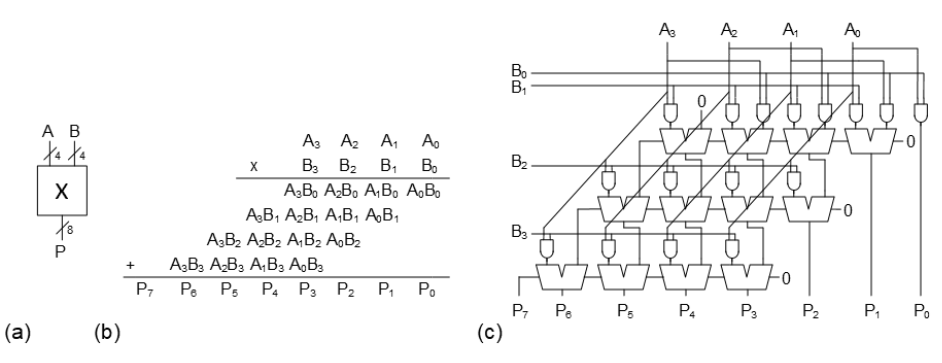
\includegraphics[width=0.8\textwidth]{exercise-26-multiplication-4-by-4}
		\caption{Exercise 26: 4 by 4 multiplier}
		\label{exercise-26-multiplication-4-by-4}
	\end{figure}
\end{ex}

\begin{sol}
	All partial products are computed simultaneously, which accounts for 1 AND gate.
	Then, since $P_7$ depends on the results of the previous carries, it is on the
	critical path. From the function and the circuit implementation, there are 8
	adders on the critical path. That is, the delay is
	\begin{align*}
		t_{\text{MULT}, 4\times 4}=t_{\text{AND}}+8t_{FA}
	\end{align*}
	In an $N\times N$ multiplier, we would have $N-1$ levels of adders.There are
	2 adders of each level on the critical path, except that the last level's
	adders are all on the critical path. That is:
	\begin{align*}
		t_{\text{MULT}, N\times N}&=t_{\text{AND}} + ((N-2)\cdot 2 + N)t_{FA}\\
		&=t_{\text{AND}}+(3N-4)t_{FA}
	\end{align*}
	To verify this is correct, if $N=4$, then $3\cdot 4 - 4=8$.
\end{sol}

\begin{ex}{5.29}
	A \emph{sign extension unit} extends a two's complement number from $M$ to $N$
	($N>M$) bits by copying the most significant bit of the input into the upper
	bits of the output (see section 1.4.6). It receives an $M$-bit input $A$ and produces
	an $N$-bit output $Y$. Sketch a circuit for a sign extension unit with a 4-bit input
	and an 8-bit output. Write the HDL for your design.
\end{ex}

\begin{sol}
	See Figure~\ref{05-29-sign-extension-unit-4-to-8-bits}.
	\begin{figure}
		\centering
		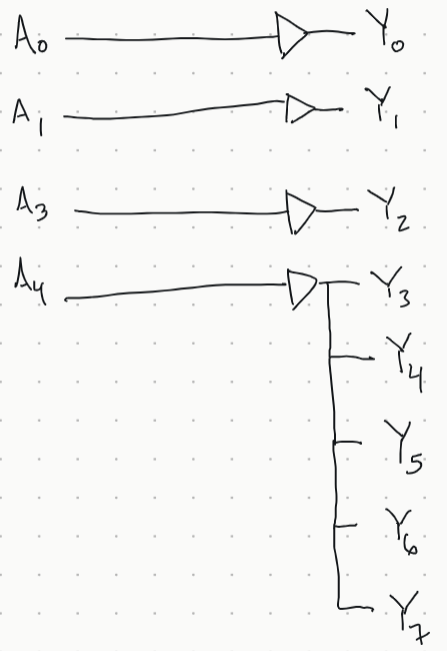
\includegraphics[width=0.3\textwidth]{05-29-sign-extension-unit-4-to-8-bits}
		\caption{Exercise 29: Sign Extension Unit (4 bits to 8 bits)}
		\label{05-29-sign-extension-unit-4-to-8-bits}
	\end{figure}
	See also the code listing \texttt{./hdl/29-sign-extension-4-8/sign\_extension\_4\_8.vhd}:
	\lstinputlisting{./hdl/29-sign-extension-4-8/sign\_extension\_4\_8.vhd}
\end{sol}

\begin{ex}{5.30}
	A \emph{zero extension unit} extends an unsigned number from $M$ to $N$
	bits ($N>M$) by putting zeros  into the upper bits of the output 
	(see section 1.4.6). Sketch a circuit for a zero extension unit with a 4-bit
	input and an 8-bit output. Write the HDL for your design.
\end{ex}

\begin{sol}
	See Figure~\ref{exercise-05-30-zero-extension-unit}.
	\begin{figure}
		\centering
		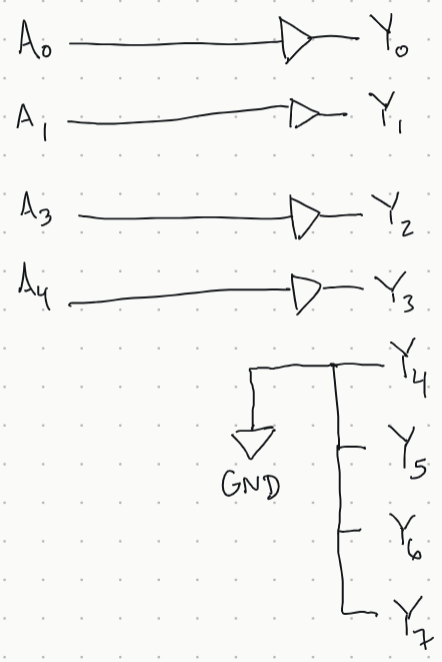
\includegraphics[width=0.3\textwidth]{exercise-05-30-zero-extension-unit}
		\caption{Exercise 30: Zero Extension Unit (4 bits to 8 bits)}
		\label{exercise-05-30-zero-extension-unit}
	\end{figure}
	See also the code listing \texttt{./hdl/30-zero-extension-4-8/zero\_extension\_4\_8.vhd}:
	\lstinputlisting{./hdl/30-zero-extension-4-8/zero\_extension\_4\_8.vhd}
\end{sol}

\begin{ex}{5.31}
	Compute $111001.000_2/001100.000_2$ in binary using the standard division
	algorithm from elementary school. Show your work.
\end{ex}

\begin{sol}
	See Figure~\ref{exercise-31-binary-long-division}. Note that the standard
	subtraction, we add $\bar{B}+1$ at each step.
	\begin{figure}
		\centering
		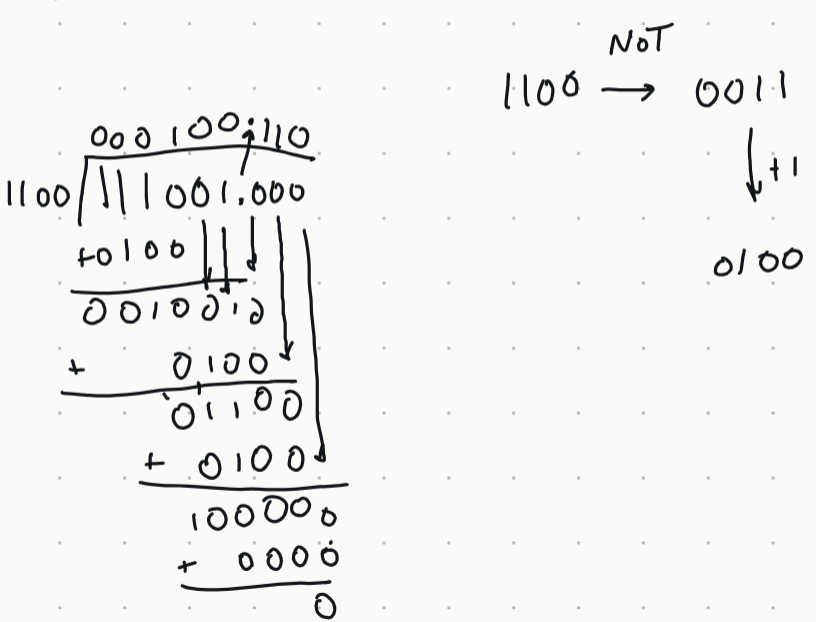
\includegraphics[width=0.5\textwidth]{exercise-31-binary-long-division}
		\caption{Exercise 31: Binary Long Division}
		\label{exercise-31-binary-long-division}
	\end{figure}
\end{sol}

\begin{ex}{5.32}
	What is the range of numbers that can be represented by the following number
	systems?
	\begin{enumerate}[label=(\alph*)]
		\item U12.12 format (24-bit unsigned fixed-point numbers with 12 integer
		bits and 12 fraction bits).
		\item 24-bit sign/magnitude fixed-point numbers with 12 integer bits and
		12 fraction bits.
		\item Q12.12 format (24-bit two's complement fixed-point numbers with 12
		integer bits and 12 fraction bits).
	\end{enumerate}
\end{ex}

\begin{sol}
	\begin{enumerate}[label=(\alph*)]
		\item The smallest number is 0. The highest is asserts 12 integer bits and 12 fraction bits.
		Since $\sum_{i=0}^{11}2^i=2^{12}-1$, and $\sum_{i=1}^{12}2^{-i}=1-2^{-12}$,
		so the maximum value is $2^{12}-1+1^{-12}=2^{12}-2^{-12}$.
		\item In this case, the the maximum value is the same, obtained when all but the sign bit
		are 1: $2^{12}-2^{-12}$. For the smallest number, all bits are 1 (including the sign bit).
		The minimum value is the negative of the maximum value.
		\item Maximum is $2^{12}-2^{-12}$, and the minimum value is $-2^{12}+2^{-12}-1$, which is
		1 lower than the maximum value.
	\end{enumerate}
\end{sol}

\begin{ex}{5.33}
	Express the following base 10 numbers in 16-bit fixed point sign/magnitude
	format with eight integer bits and eight fraction bits. Express your
	answer in hexadecimal.
	\begin{enumerate}[label=(\alph*)]
		\item $-13.5625$
		\item $42.3125$
		\item $-17.15625$
	\end{enumerate}
\end{ex}

\begin{sol}
	\
	\begin{enumerate}[label=(\alph*)]
		\item To do the conversion, we start with $13.5625$, and do repeated division
		by powers of $2$, subtracting each time:
		\begin{align*}
			13.5625&\geq 2^{3}\implies 1\\
			5.5625&\geq 2^{2}\implies 1\\
			1.5625&< 2^{1}\implies  0\\
			1.5625&\geq 2^{0} \implies 1\\
			0.5625&\geq 2^{-1}\implies 1\\
			0.0625& < 2^{-2}\implies 0\\
			0.0625&<2^{-3}\implies 0\\
			0.0625&\geq 2^{-4} \implies 1\\
			0&
		\end{align*}
		Therefore, $13.5625_{10}=0000 1101.10010000 _2$. 
		For 16-bit fixed-point sign/magnitude format, we use 8 fraction bits and 8
		integer bits, setting the sign bit to 1 for negative numbers. Hence, the number is
		\begin{align*}
			1000 1101.1001 0000_2=\texttt{0x8D.90}
		\end{align*}
		\item We repeat the same steps:
		\begin{align*}
			42.3125&\geq 2^{5}\implies 1\\
			10.3125& < 2^{4}\implies 0\\
			10.3125&\geq 2^{3}\implies 1\\
			2.3125&< 2^{2}\implies 0\\
			2.3125&\geq 2^{1}\implies 1\\
			0.3125&< 2^{0}\implies 0\\
			0.3125& < 2^{-1}\implies 0\\
			0.3125&\geq 2^{-2}\implies 1\\
			0.0625&<2^{-3}\implies 0\\
			0.0625&\geq 2^{-4}\implies 1\\
			0&
		\end{align*}
		Therefore, $42.3125_{10}=0010 1010.0101=\texttt{0x2A.50}$.
		\item Finally, same as part (a), though I will skip some powers:
		\begin{align*}
			17.15625&\geq 2^{4}\implies 1\\
			1.15625&\geq 2^{0}\implies 1\\
			0.15625&\geq 2^{-3}\implies 1\\
			0.03125&\geq 2^{-5}\implies 1
		\end{align*}
		Therefore, $17.15625_{10}=10001.00101_2$, so its negative has a 1 as a sign bit,
		meaning $-17.15625_{10}=1001 0001.0010 1000_2=\texttt{0x91.28}$.
	\end{enumerate}
\end{sol}

\begin{ex}{5.35}
	Express the base 10 numbers in Exercise 5.33 in Q8.8 format (16-bit fixed-point
	two's complement format with eight integer bits and eight fraction bits).
	Express your answer in hexadecimal.
\end{ex}

\begin{sol}
	\begin{enumerate}[label=(\alph*)]
		\item Recall from Exercise 5.33 that $13.5625_{10}=0000 1101.1001 0000_2$, and hence,
		in two's complement we have $-13.5625_{10}= 1111 0010 . 0111 0000_2=\texttt{0xF2.70}$.
		\item Same as Exercise 33: $42.3125_{10}=0010 1010.0101=\texttt{0x2A.50}$.
		\item Recall from Exercise 5.33 that $17.15625_{10}=0001 0001.0010 1000_2$. When
		negating it using two's complement, we get
		$-17.15625_{10}=1110 1110.1101 1000_2=\texttt{0xEE.D8}$.
	\end{enumerate}
\end{sol}


\begin{ex}{5.37}
	Express the base 10 numbers in Exercise 5.33 in IEEE 754 single-precision
	floating-point format. Express your answer in hexadecimal.
\end{ex}

\begin{sol}
	The IEEE 754 single-precision format uses 32 bits, where
	\begin{itemize}
		\item 1 bit is assigned to most significant bit for sign
		\item 8 bits are assigned to a biased exponent
		\item 23 bits are assigned to the fraction portion
	\end{itemize}
	\begin{enumerate}[label=(\alph*)]
		\item Recall that $13.5625_{10}=0000 1101.1001 0000 _2$ from Exercise 5.33.
		Since the number is negative, the sign bit will be 1. By moving the decimal
		place to the left 3 times, we get $1.1011001\times 2^{3}$, meaning the
		exponent is $3$ and the mantissa is $1101 1001_2$ (with more 0s padded until
		it has a total of 23 bits). Since the leading 1 is implicit and is not to be
		included in the mantissa, we remove it to have $101 1001_2$. Finally,
		the biased exponent is the original exponent plus a constant bias, which
		for a 32-bit floating-point number is $127$. That is: $3+127=130=1000 0010_2$,
		which is the biased exponent. Hence the IEEE 754 single-precision floating point
		format representation of $-13.5625_{10}$ is

		\begin{center}
			\begin{tabular}{c|c|c}
				Sign (1-bit) & Biased Exponent (8-bits) & Fraction\\
				\hline
				1 & 1000 0010 & 101 1001 0000 0000 0000 0000
			\end{tabular}
		\end{center}
		\item Recall that $42.3125_{10}=0010 1010.0101_2$. Since the number is
		positive, the sign bit is 0. By moving the decimal place left 5 times,
		we get $1.010100101_2\times 2^5$. Since the leading bit is always 1, the fraction
		bit does not use the leading bit of the mantissa, so the leading portion
		of the fraction part of the representation is $010100101$. Moreover,
		since the exponent is $5$, we bias it by adding $127$, getting $132=1000 0101_2$
		so the IEEE 754 single-point floating point representation of $42.3125_{10}$
		is:
		\begin{center}
			\begin{tabular}{c|c|c}
				Sign (1-bit) & Biased Exponent (8-bits) & Fraction\\
				\hline
				0 & 1000 0101 & 010 1001 0100 0000 0000 0000
			\end{tabular}
		\end{center}
		\item We are converting  $-17.15625_{10}$, so the sign bit is 1.
		From Exercise 5.33, we have $17.15625_{10}=10001.00101_2$. By moving
		the decimal place left 4 times, we get $1.000100101_2\times 2^4$. Removing
		the leading bit, we get the leading fraction part which is $000 1001 01_2$.
		We add $127$ to the exponent to bias it, getting $4+127=131=1000 0100_2$.
		The IEEE 754 single-point floating point representation of $-17.15625_{10}$ is
		\begin{center}
			\begin{tabular}{c|c|c}
				Sign (1-bit) & Biased Exponent (8-bits) & Fraction\\
				\hline
				1 & 1000 0100 & 000 1001 0100 0000 0000 0000
			\end{tabular}
		\end{center}
	\end{enumerate}
	
\end{sol}

\begin{ex}{5.39}
	Convert the following Q4.4 (two's complement binary fixed-point numbers)
	to base 10. The implied binary point is explicitly shown to aid in your
	interpretation.
	\begin{enumerate}[label=(\alph*)]
		\item 0101.1000
		\item 1111.1111
		\item 1000.0000
	\end{enumerate}
\end{ex}

\begin{sol}
	\
	\begin{enumerate}[label=(\alph*)]
		\item Since the leading bit is 0, we have a positive number. Then
		we add the powers of $2$:
		\begin{align*}
			0101.1000_2=2^{2}+2^{0}+2^{-1}=5.5_{10}
		\end{align*}
		\item Since the leading bit is 1, this is a negative number. We take its
		two's complement by inverting all of the bits and adding 1, yielding:
		$0000.0001_2$. Then we convert it to base 10:
		\begin{align*}
			0000.0001_2=2^{-4}=-0.0625_{10}
		\end{align*}
		\item Since the leading bit is 1, the number is negative. We take its
		two's complement by inverting all of the bits and adding 1, yielding:
		$1000.0000_2$. Then we convert it to base 10:
		\begin{align*}
			1000.0000_2&=-2^{3}=-8_{10}
		\end{align*}
	\end{enumerate}
\end{sol}

\begin{ex}{5.41}
	When adding two floating-point numbers, the number with smaller exponent is
	shifted. Why is this? Explain in words and give an example to justify your
	explanation.
\end{ex}

\begin{sol}
	When fraction bits of both numbers are converted to a mantissa, they both have
	24 bits (a 1 to the left of the decimal, followed by a decimal point, followed
	by 23 bits). However, the numbers do not have the same order of magnitude; they
	differ by an order of magnitude indicated by their exponent, which must be
	accounted for. Rather than move both numbers according to their order of magnitude,
	we express the smaller number in the same order of magnitude as the larger number.
	We do so by taking the difference of their exponents. We shift the smaller number
	a number of places equals to the absolute value of the difference. Then, the exponent
	used for both is the larger of the two. For example, consider
	\begin{align*}
		3.87\times 10^{3}+2.41\times 10^{5}
	\end{align*}
	in base 10. We cannot just add 2.81 and 3.87. Instead, since their exponents differ
	by -22, the we shift the decimal in 3.87 by 2 units left to make it $0.0387\times 10^{5}$.
	Now we have
	\begin{align*}
		0.0387\times 10^{5}+2.41\times 10^{5}=2.4487\times 10^5
	\end{align*}
	A similar case holds in base 2. For example, recall from Exercise 5.33 that the
	floating-point representation of $42.3125_{10}$ is
	\begin{center}
		\begin{tabular}{c|c|c}
			Sign (1-bit) & Biased Exponent (8-bits) & Fraction\\
			\hline
			0 & 1000 0101 & 010 1001 0100 0000 0000 0000
		\end{tabular}
	\end{center}
	and the floating-point representation of $-17.15625_{10}$ is
	\begin{center}
		\begin{tabular}{c|c|c}
			Sign (1-bit) & Biased Exponent (8-bits) & Fraction\\
			\hline
			1 & 1000 0100 & 000 1001 0100 0000 0000 0000
		\end{tabular}
	\end{center}
	To add them, we follow the 8-step process described in Section 5.3.2:
	\begin{enumerate}
		\item Extract the exponent and fraction bits:
		\begin{center}
			\begin{tabular}{|c|c|c|}
				\hline
				0 & 1000 0101 & 010 1001 0100 0000 0000 0000\\
				\hline
				1 & 1000 0100 & 000 1001 0100 0000 0000 0000\\
				\hline
			\end{tabular}
		\end{center}
		\item Then, prepend leading 1 to form the mantissa:
		\begin{center}
			\begin{tabular}{|c|c|c|}
				\hline
				0 & 1000 0101 & \textbf{1}.010 1001 0100 0000 0000 0000\\
				\hline
				1 & 1000 0100 & \textbf{1}.000 1001 0100 0000 0000 0000\\
				\hline
			\end{tabular}
		\end{center}
		\item We compare exponents, i.e., subtract them:
		\begin{center}
			\begin{tabular}{|c|c|c|}
				\hline
				0 & 1000 0101 & 1.010 1001 0100 0000 0000 0000\\
				\hline
				1 & 1000 0100 & 1.000 1001 0100 0000 0000 0000\\
				\hline
				{} & \text{1}
			\end{tabular}
		\end{center}
		\item The result of the previous step was 1, meaning that the second operand has a smaller
		exponent and order of magnitude; this is correct, since $42.3125_{10}$ uses
		a base 2 exponent of $5$, while $-17.15625_{10}$ uses a base 2 exponent of
		$4$. Hence, we shift the base 2 representation of $-17.15625_{10}$ right
		by 1 unit and change its exponent to match the larger 1:
		\begin{center}
			\begin{tabular}{|c|c|c|}
				\hline
				0 & 1000 0101 & 1.010 1001 0100 0000 0000 0000 0\\
				\hline
				1 & 1000 0101 & 0.100 0100 1010 0000 0000 0000 0\\
			\end{tabular}
		\end{center}
	\end{enumerate}
	The addition can then take place in the next step, keeping in mind that the second
	operand is negative.
\end{sol}

\begin{ex}{5.44}
	Expand the steps in Section 5.3.2 for performing floating-point addition to work
	for negative as well as positive floating-point numbers.
\end{ex}

\begin{sol}
	\
	\begin{enumerate}
		\item Extract exponent and fraction bits.
		\item Prepend leading 1 to form the mantissa.
		\item Compare exponents.
		\item Shift smaller mantissa if necessary.
		\item Take two's complement of first operand's mantissa if its sign bit is 1.
		\item If the second operand is positive, negative it using the two's complement.
		Otherwise, leave it unchanged.
		\item Add the mantissas.
		\item Normalize mantissa and adjust exponent if necessary.
		\item Round result.
		\item Assemble exponent and fraction back into floating-point numbers.
	\end{enumerate}
\end{sol}

\begin{ex}{5.45}
	Consider IEEE 754 single-precision floating-point numbers.
	\begin{enumerate}[label=(\alph*)]
		\item How many numbers can be represented by the IEEE 754 single-precision
		floating-point format? You need not count $\pm\infty$ or NaN.
		\item How many additional numbers could be represented if $\pm \infty$ and
		NaN were not represented?
		\item Explain why $\pm \infty$ and NaN are given special representations.
	\end{enumerate}
\end{ex}

\begin{sol}
	\begin{enumerate}[label=(\alph*)]
		\item The 32-bit representation  means that $2^{32}$ binary sequences can be
		represented. We subtract 1 because $0$ has a positive and negative representation.
		We subtracting $2$ due to $\pm \infty$. Next, note that NaN occurs when
		all exponents bits are asserted and the fraction bit is nonzero, regardless
		of the sign bit. Since the fraction portion has 23 bits, there are $2^{23}-1$
		nonzero combinations. we double it to account for the don't care in the sign
		bit, so there are $2^{24}-2$ ways to represent NaN. Hence, the total amount
		of numbers that can be represented with IEEE 754 single-precision floating point
		format is
		\begin{align*}
			2^{32}-1-2-(2^{24}-1)=2^{32}-2^{24}-2=4,278,190,078_{10}
		\end{align*}
		\item If $\pm \infty$ and NaN were not represented, we would be able to
		represent $2^{32}-1=4,294,967,294$ numbers.
		\item It's possible for floating-point operations to yield numbers bigger than
		what can be represented with a finite set of bits. To indicate this, the
		$\pm\infty$ representations communicate that an operation caused overflow. 
		Meanwhile, NaN represents operations that do not yield a \emph{real} number.
		Their values can be used to make decisions about how to proceed with a
		calculation.
	\end{enumerate}
\end{sol}


\end{document}